\chapter[Introdução]{Introdução}

É inconcebível imaginar o mundo moderno sem software. A sua penetração é tão grande nas mais diversas áreas que seria difícil prever como o mundo seria sem o suporte e as facilidades que ele trás ao nosso dia a dia. Diante desta penetração tão grande e do seu enorme crescimento nos últimos anos, consequência do avanço tecnológico, se torna cada vez mais importante desenvolver software. O desenvolvimento de software pode possuir diferentes contextos de negócio, e com isso diferentes habilidades são exigidas dos desenvolvedores, já que cada contexto possui suas particularidades. Além disso, o ritmo acelerado do mundo moderno faz com que os contextos evoluam, e com isso as suas atividades e necessidades (requisitos) também evoluem. A mudança nos requisitos, a sua diversidade, e em algumas vezes a dificuldade em precisa-los, leva o desenvolvimento tradicional de software a ser lento e caro em contextos que estão sempre evoluindo \cite{lieberman2006}. Além disso, a limitação na capacidade de produção de software de uma organização pode levar à priorização das demandas, e como consequência áreas de negócio podem ficar sem atendimento. Diante deste cenário, se torna cada vez mais comum aplicações de software serem desenvolvidas por desenvolvedores não profissionais, pessoas que possuem expertise em um determinado domínio e que desejam suportar seus objetivos neste domínio através de uma solução computacional \cite{lieberman2006}. O Escritório do Trabalho e Estatística dos Estados Unidos fez uma previsão de que por volta de 2012, nos Estados Unidos, haveriam pouco mais de 3 milhões de programadores profissionais e mais de 55 milhões de pessoas escrevendo fórmulas e \textit{queries} em planilhas e banco de dados, para suportar seus objetivos de trabalho \cite{scaffidi2005}. Um relatório divulgado pelo \textit{Gartner} em Julho de 2011, indicou que desenvolvedores não profissionais iriam construir ao menos 25 \% das novas aplicações de negócio em 2014 \cite{paterno2013}. Diante deste cenário, um modelo de desenvolvimento de software centrado no usuário final cada vez mais vem ganhando força. O \textit{End User Development} - EUD tem como objetivo oferecer meios para que os usuários finais, que não são especialistas em programação, possam desenvolver aplicações de software. O EUD pode ajudar a aumentar a capacidade produtiva do departamento de TI de uma organização, bem como reduzir custos com o desenvolvimento de aplicações de negócio.

O serviço público brasileiro, por ter natureza administrativa, apresenta grande demanda por desenvolvimento de software. Porém a limitada capacidade produtiva da área de TI e o excesso de burocracia para o aumento da mesma, que é feita através de concursos ou de contratos terceirizados, acaba contribuindo para que as demandas das áreas de negócio consideradas menos prioritárias sejam deixadas de lado \cite{artigoTcuGovTI}. O uso de planilhas e o desenvolvimento de aplicações clandestinas sem nenhuma documentação e padrão, por essas unidades de negócio, promove o desconhecimento de soluções informatizadas por parte da alta cúpula, bem como a duplicidade de esforços pelas unidades \cite{slideTCU}. Nesse sentido, alguns órgãos da administração pública federal veem reconhecendo esses esforços feitos informalmente pelas áreas de negócio, e começaram a adotar o modelo EUD, com algumas adaptações, para tentar contornar os problemas relatados. Os órgãos vem chamando esse modelo de modelo de desenvolvimento descentralizado, uma espécie de EUD onde o usuário final não é necessariamente quem desenvolve as aplicações. Geralmente estagiários da área de TI são contratados, para que eles possam ser alocados nas unidades de negócio do órgão, de forma que eles desenvolvam as aplicações junto à área de negócio, com a consultoria técnica da área de TI \cite{slideTCU}. Uma iniciativa bem sucedida de desenvolvimento descentralizado já foi implantada em um órgão da administração pública federal, com um relato de alta satisfação dos usuários. Apesar disso, ainda existem algumas dificuldades no desenvolvimento por parte dos estagiários, que não possuem um guia/processo que os oriente durante todo o ciclo de desenvolvimento. Por serem estagiários, muitos acabam seguindo a forma de desenvolvimento e os padrões que acreditam serem os melhores, o que acaba colocando em dúvida a qualidade das aplicações desenvolvidas. 

O objetivo geral deste trabalho é desenvolver uma solução de apoio ao desenvolvimento EUD (descentralizado) para um orgão público federal, agregando recursos que promovam a qualidade dos sistemas desenvolvidos, a partir de princípios e conceitos de engenharia de software.

Considerando o objetivo geral, foram definidos os seguintes objetivos específicos:

\begin{enumerate}
\item Entender o contexto do EUD no orgão público alvo.
\item Diagnosticar os problemas no desenvolvimento de aplicações baseado em EUD.
\item Selecionar as práticas da engenharia de software que sejam adequadas à solução dos problemas encontrados e ao contexto.
\item Elaborar o modelo conceitual da solução de apoio.
\item Construir a solução de apoio.
\item Selecionar um projeto para a aplicação da solução.
\item Aplicar a solução de apoio no projeto selecionado.
\item Relatar os resultados obtidos.
\end{enumerate}


\begin{comment}
Apesar disso, existem ainda algumas dificuldades no desenvolvimento por parte dos estagiários desenvolvedores, como a falta de padronização e o que demonstra a necessidade de a elaboração de um processo embasado por princípios em conceitos da engenharia de software, ao mesmo tempo que não seja custoso aos desenvolvedores, já que iria contra a flexibilidade que preconiza o modelo EUD. 

\citeonline{lieberman2006} relatou que um dos objetivos da interação humano-computador, além de desenvolver sistemas que são fáceis de usar, seria desenvolver sistemas que são fáceis de desenvolver.
\end{comment}

\chapter[Referencial Teórico]{Referencial Teórico}

Esta seção apresenta o referencial que embasa este trabalho, de forma a demonstrar o resultado da revisão de literatura feita. O referencial teórico é o meio em que o autor do trabalho demonstra o seu conhecimento sobre uma determinada área de estudo (teorias, vocabulários, variáveis chave, fenômenos, métodos e história) \cite{randolph2009}.

O referencial teórico é composto dos seguintes assuntos: \textit{End User Development}.


\section{\textit{End User Development}}

\textit{End User Development} (Desenvolvimento por usuário final) é um modelo de desenvolvimento de software onde o usuário final é o principal responsável pela construção do software. \citeonline{lieberman2006} define o \textit{End User Development} (EUD) como um conjunto de métodos, técnicas e ferramentas que permitam aos usuários de sistemas de software, que agem como desenvolvedores de software não profissionais, em algum ponto criar, modificar ou estender um artefato de software. Dentre as motivações para este modelo de desenvolvimento, destacam-se a diversidade e a mutabilidade dos requisitos, bem como a dificuldade em precisa-los em contextos que evoluam com uma alta frequência, o que pode levar o desenvolvimento tradicional a consumir muito tempo e atingir um alto custo \cite{lieberman2006}. Além disso, uma organização que possui uma demanda por informatização dos seus processos de trabalho, por parte das suas diferentes áreas de negócio, superior a capacidade produtiva da área de TI, pode não conseguir atender certas áreas por conta das priorizações das demandas \cite{artigoTcuGovTI}. O EUD acelera as respostas às mudanças e contorna o problema de precisão dos requisitos, porque os usuários finais geralmente são especialistas no domínio em que estão inseridos, ou seja, são os detentores dos requisitos da solução computacional \cite{fischer2004}. O fato de cada usuário final ser um potencial desenvolvedor também contribui para um aumento da capacidade produtiva da TI.

Para que o desenvolvimento seguindo este modelo possa ocorrer é necessário que existam meios para que o usuário final possa desenvolver e adaptar o software, e para tanto a tecnologia envolvida deve diminuir o esforço cognitivo necessário para a construção do software, através da aproximação conceitual entre as ações do mundo real e as do mundo da programação \cite{fischer2004}. Os usuários finais geralmente não possuem habilidades de um profissional da área de software, e também não estão interessados em construir sistemas no mesmo nível que esses profissionais, por isso é necessário que a tecnologia usada no desenvolvimento alinhe a complexidade relacionada a esta atividade com as habilidades do usuário final. A motivação dos usuários finais é algo essencial para o favorecimento deste modelo, e fatores como o empoderamento, a velocidade de desenvolvimento, a flexibilidade e o controle influênciam diretamente na motivação desses usuários.

O principal objetivo do EUD é oferecer meios para que os usuários finais consigam desenvolver e adaptar software \cite{lieberman2006}. Desta maneira, as aplicações preparadas para o EUD devem ser, principalmente, flexíveis, fáceis de se entender, de se usar, e de se ensinar \cite{lieberman2006}. A preocupação com a tecnologia usada neste modelo de desenvolvimento, mais especificamente na parte das linguagens de programação e aplicações de desenvolvimento, é a relação escopo de aplicação versus esforço de aprendizagem. A figura 1 ilustra a relação do escopo de aplicação e do custo de aprendizagem, para diferentes linguagens de programação e aplicações. Linguagens de programação mais tradicionais como C++ e JAVA oferecem a possibilidade de construção de software de uma grande variedade de domínios, porém a um alto custo associado ao esforço de aprendizagem. Outras linguagens possuem um menor esforço de aprendizagem, ao custo de uma limitação no escopo de aplicação. As linguagens ou aplicações de desenvolvimento ideais para o EUD são as que possuem um alto escopo de aplicação e um baixo esforço de aprendizagem \cite{fischer2004}. As que existem atualmente só utilizam uma pequena parte do potencial do EUD, com algumas falhas \cite{paterno2013}.

\begin{figure}[h]
	\centering
	\label{fig01}
		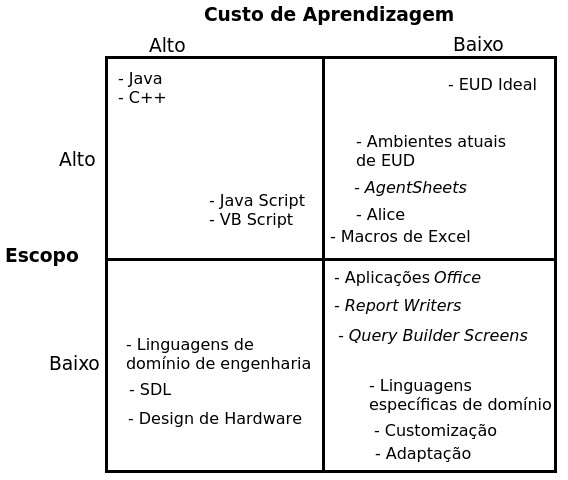
\includegraphics[scale=0.8]{figuras/trade_off_eud_editado}
	\caption{Relação escopo de aplicação e custo de aprendizagem}
\end{figure}
\pagebreak

\citeonline{lieberman2006} classifica as atividades do usuário final em dois tipos:

\begin{enumerate}
\item \textbf{Parametrização ou Customização:} São atividades que permitem o usuário escolher comportamentos, apresentações e mecanismos  alternativos, que já existem dentro de uma aplicação.

\item \textbf{Criação e modificação de programas:} São atividades que implicam na criação ou modificação de artefatos de software. Macros e linguagens de \textit{script} são exemplos deste tipo de atividade.
\end{enumerate}


\chapter[Metodologia]{Metodologia}

\citeonline{gil2002} classifica as pesquisas científicas em três grandes grupos, segundo os seus objetivos gerais: exploratórias, descritivas e explicativas.

Destes três grupos, a pesquisa exploratória, em particular, tem como objetivo proporcionar o aprimoramento e/ou a descoberta de idéias, a respeito de um determinado problema. Proporcionando uma maior familiaridade com o problema, esse tipo de pesquisa o torna mais explícito e contribui para a construção de hipóteses em cima do mesmo. Por conta disso, a pesquisa exploratória possui um caráter flexível em seu planejamento, e geralmente assume as formas de pesquisa bibliográfica ou estudo de caso \cite{gil2002}.

O estudo de caso consiste no estudo profundo e exaustivo de um ou mais objetos, de forma a obter conhecimento amplo e detalhado sobre o mesmo. Segundo \citeonline{yin2001estudo} o estudo de caso é a abordagem mais adequada para a investigação de um fenômeno em seu contexto real, onde os limites entre este fenômeno e o seu contexto não são claramente percebidos. Os propósitos do estudo de caso são \cite{gil2002}:

\begin{itemize}
\item Explorar situações de contextos reais onde os limites não estão claramente definidos.
\item Preservar o caráter unitário do objeto.
\item Descrever a situação do contexto do qual esta sendo feita a investigação.
\item Desenvolver teorias e formular hipóteses.
\item Determinar as causas de um determinado fenômeno onde a complexidade não permite o uso de levantamentos e experimentos.
\end{itemize}

Existem diversos métodos de coleta de dados para suportar os propósitos de um estudo de caso, e um dos métodos comumente usados nos estudos de caso na engenharia de software é a entrevista \cite{caseStudySE}. Quase todos os estudos de caso envolvem algum tipo de entrevista, seja para a finalidade primária de coleta dados, seja para uma validação de outros tipos de dados \cite{caseStudySE}. A entrevista é caracterizada como um método de coleta de dados onde o pesquisador esta em contato direto com os entrevistados e como um método de coleta de dados em tempo real \cite{caseStudySE}. O diálogo entre o entrevistador e o entrevistado é guiado por um conjunto de perguntas, que podem ser classificadas como abertas ou fechadas \cite{caseStudySE}. As perguntas abertas permitem uma maior gama de respostas e relatos de problemas, por parte do entrevistado. Já as perguntas fechadas oferecem alternativas mais limitadas, se comparadas as perguntas abertas. Ambos os tipos de perguntas são baseadas nos tópicos de interesse relacionados ao estudo de caso. 

Segundo \cite{caseStudySE}, a entrevista pode ser classificada em três categorias diferentes:
\begin{enumerate}
\item \textbf{Não-estruturada}: As perguntas são formuladas de forma aberta e de acordo com os interesses do pesquisador. A conversa durante a entrevista irá se desenvolver de acordo com os interesses do entrevistado e do entrevistador.
\item \textbf{Semi-estruturada}: As questões planejadas não são necessariamente perguntadas na ordem em que estão listadas, tendo o desenvolvimento da conversa influência direta na ordem em que as perguntas são feitas ao entrevistado. Além disso, esse tipo de pesquisa permite o improvisamento e a exploração de problemas levantados durante a conversa. É comum em estudos de caso em engenharia de software.
\item \textbf{Completamente estruturada}: Todas as perguntas são detalhadamente planejadas de antemão e são feitas exatamente na ordem em que estão listadas. Esse tipo de entrevista se assemelha a \textit{surveys} baseados em questionários, pois se trata de perguntas fechadas.
\end{enumerate}
	
Uma vez que os dados são coletados, o foco se volta para a análise e interpretação dos mesmos. O objetivo desta etapa é derivar conclusões dos dados, buscando a compreensão e a formação de padrões em cima dos mesmos, através de uma cadeia de evidência. Uma cadeia de evidência significa que o leitor pode chegar aos mesmos resultados e conclusões em cima dos dados coletados \cite{caseStudySE}. A análise e interpretação dos dados pode ser divida nos seguintes procedimentos \cite{caseStudySE}:

\begin{enumerate}
\item Os dados são codificados de forma que a cada pedaço do texto, que pode ser uma linha ou um parágrafo por exemplo, é atribuído um código que pode representar um certo tema, uma área, uma construção e assim por diante. Observa-se que um pedaço de texto pode possuir mais de um código e um código pode estar associado a mais de um pedaço de texto.
\item Identificar um conjunto de hipóteses em cima dos dados codificados.
\item Formar um conjunto de generalizações/conclusões.
\item Relatar os resultados.
\end{enumerate}

\section{Metodologia Adotada}

A metodologia adotada para este trabalho foi o estudo de caso, já que foi necessário realizar um diagnóstico para a construção da solução de apoio, e o método utilizado no estudo de caso foi a entrevista, por ser um método bastante comum neste tipo de metodologia. 

A entrevista elaborada pode ser classificada como semi-estruturada, já que as perguntas foram feitas na ordem em que foram planejadas e improvisos foram feitos, de forma a coletar dados adicionais que julgou-se serem interessantes ao estudo. Categorias de perguntas foram elaboradas, de forma a auxiliar na formulação das perguntas.

As categorias elaboradas foram:

\begin{itemize}
\item \textbf{Descrição do desenvolvedor} 

- Objetivo: Obter informações sobre o perfil dos desenvolvedores.
\item \textbf{Papel do desenvolvedor}

- Objetivo: Obter informações sobre o papel do desenvolvedor no órgão.
\item \textbf{Efetividade do curso}

- Objetivo: Obter informações sobre a preparação dos novos desenvolvedores.
\item \textbf{Requisitos}

- Objetivo 1: Obter informações sobre como se dá o levantamento de requisitos nos departamentos da instituição.

- Objetivo 2: Obter informações de como é armazenado e gerenciado os requisitos do sistema a ser desenvolvido.

- Objetivo 3: Obter informações de como é englobado as mudanças de requisitos ao sistema.
\item \textbf{\textit{Design}}

- Objetivo: Obter informações sobre como é realizado a modelagem (arquitetura) do sistema.
\item \textbf{Codificação}

- Objetivo 1: Obter informações sobre a depuração de erros do sistema.

- Objetivo 2: Obter informações sobre estilos de codificação.

- Objetivo 3: Obter informações sobre o ambiente de codificação.

\item \textbf{Teste}

- Objetivo: Obter informações sobre a realização dos testes, bem como a forma de realiza-los.
\item \textbf{Implantação}

- Objetivo: Obter informações sobre a migração, para a produção, do sistema.
\end{itemize}

A partir das categorias definidas, foram derivadas as perguntas relacionadas a cada categoria, de forma que estivessem alinhadas ao contexto do desenvolvimento descentralizado. As perguntas elaboradas para a entrevista podem ser vistas no Anexo A.


\begin{comment}
O conjunto de etapas que podem ser seguidos na maioria das pesquisas classificadas como estudo de caso, bem como uma breve descrição destas etapas são apresentados a seguir \cite{gil2002}.

\begin{enumerate}
\item \textbf{Formulação do problema.}

Constitui a primeira etapa da pesquisa. O problema constitui um fato no qual se deseja aprofundar, de forma a fazer uma descrição de um determinado fenômeno, ou descobrir respostas as causas deste fenômeno. Cuidado deve ser tomado para que o tema seja passível de verificação.

\item Definição da unidade-caso a ser estudada.

A unidade-caso refere-se a um indivíduo num contexto definido. Possui três

\item Determinação do número de casos
\item Elaboração do roteiro.
\item Coleta dos dados.
\item Análise dos dados coletados.
\item Elaboração do relatório.
\end{enumerate}
\end{comment}
